\section*{Merge: Experimentación}

Antes de comenzar a testear, supusimos que la performance de nuestros programas en assembler iban a ser muy superiores a las de C. Creemos esto dado que vamos a aprovecharnos mejor de las utilidades de SSE que lo que puede hacer un compilador. 

Esperamos también que la performance mejore aún más en la segunda implementación, dado que todas las operaciones las realizamos con enteros en vez de con punto flotante.


\begin{figure}[!hbt] 
  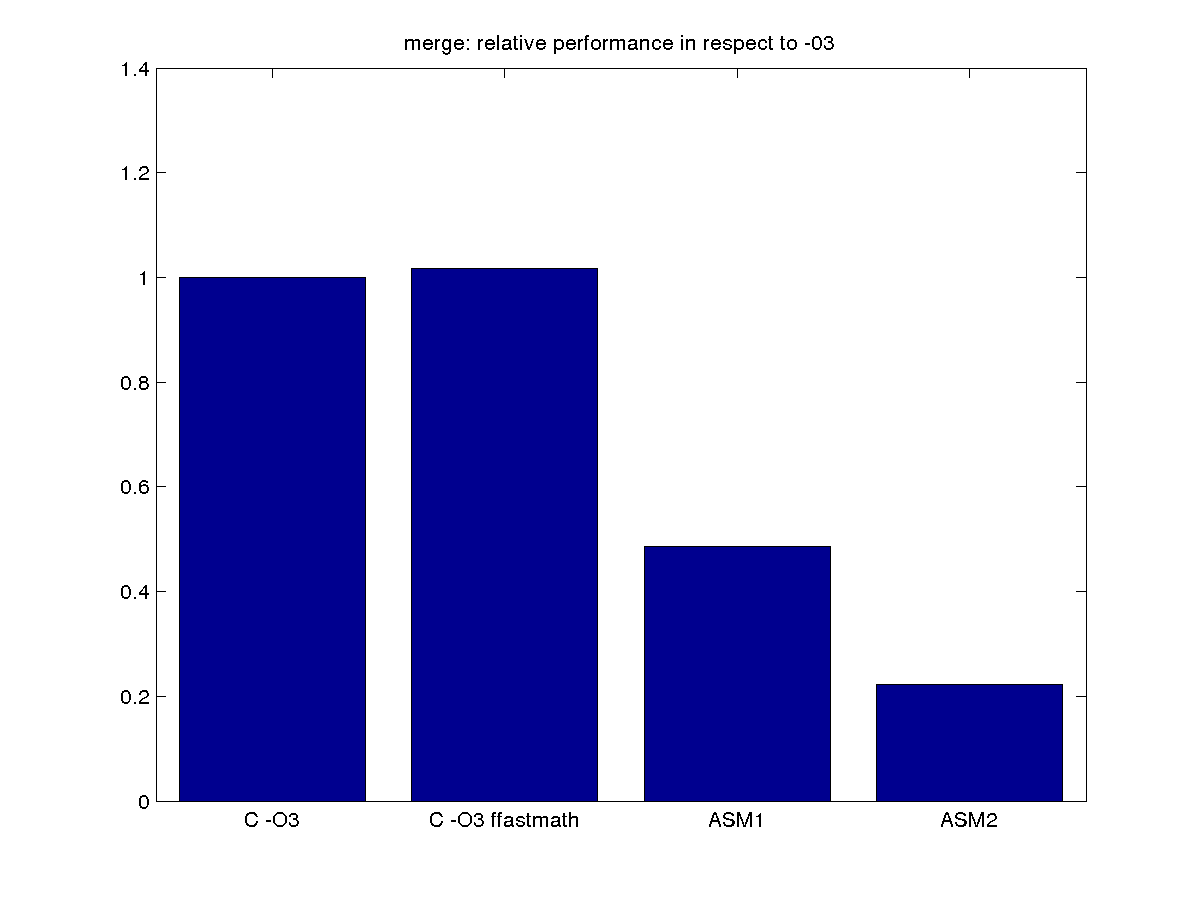
\includegraphics[width=10cm]{merge-random-uniform-pixel-fixed-size_barchart.png}
	\centering
\end{figure}



Viendo los resultados, confirmamos nuestras hipótesis. De hecho, la performance de nuestros programas son mejores que las esperadas.

Como puede verse en los gráficos de escalabilidad, la performance de todos los algoritmos depende linealmente de la cantidad de píxeles de la imagen, sin embargo lo que cambia entre las diferentes implementaciones es la pendiente de esta función lineal.

La performance no depende de la imagen, dado que la operación que se realiza siempre es la misma, sin depender de los píxeles en cuestión.
Sin embargo, hay una cuestión con el error. Si el $\alpha$ que nos pasan por parámetro tiene muchos decimales detrás de la coma, es muy probable, y de hecho pasa, que nuestra segunda implementación en assembler pierde precisión frente a la implementacion de C. Esto fue explicado anteriormente, sin embargo creímos pertinente nombrarlo.

La única mejora que se nos ocurre para el código propuesto de assembler es, si supieramos que el inicio de la matriz está alineado a 16 bytes, entonces podríamos levantar de a 4 pixeles y analizarlos todos juntos (haciendo una especie de loop unrolling, es decir, teniendo 4 ciclos normales dentro de 1).
Esto es posible que mejore la performance, sin embargo es necesario como precondición que la matriz esté alineada a 16 bytes, ya que si no lo está y usamos una instrucción para leer alineado, los resultados serán desastrosos.

La comparación entre el programa de C y el de assembler no es lo suficientemente justa. Esto se debe a que la versión de C por cada pixel, tiene 3 accesos a memoria, mientras que nuestra impelementación tiene un acceso a memoria por píxel. Esto genera obviamente un speedup enorme, sobre todo en computadoras con memoria de velocidad limitada.
Aunque es posible que la gran mayoría de los accesos sean a cache, la performance ganada es significativa.

El acceso a memoria en nuestros códigos de assembler es lo mínimo indispensable. La única mejora que se podría hacer con respecto al acceso a memoria es lo que fue nombrado anteriormente es la idea de hacer un unroll del loop y leer de a 4 pixeles, pero creemos que la performance no mejorará significativamente.

La diferencia entre operar con punto flotante y con enteros es significativa. Aunque ambas implementaciones en assembler son mucho mas rápidas que la implementación de C, la que opera con enteros es nuevamente (bastante) más rápida que la que opera con punto flotante. Esto se debe a que en general las operaciones con enteros son mucho mas rápidas que las de punto flotante.







